\documentclass[main.tex]{subfiles}
\begin{document}
\begin{bmcsex}{Tensile response of a bar with crack localization}{e51_length_dependence}
\noindent This example demonstrates stress-strain response 
    of a bar with a single cross section exhibiting softening upon
    reaching the strength $f_t$.
 \\
\begin{center}
            
{\scriptsize 
\begin{longtable}{lrp{4cm}}\toprule
\textbf{\textsf{Model parameter}} 
& 
\textbf{\textsf{Symbol = Value [Unit]}} 
&
\textbf{\textsf{Description}}  \\\midrule \midrule
\texttt{f\_t} & $f_t$ = 2.5 [MPa] & {\footnotesize tensile strength}  \\
            \texttt{A} & $A$ = 10.0 [$\mathrm{mm}^2$] & {\footnotesize cross-sectional area}  \\
            \texttt{G\_f} & $G_\mathrm{F}$ = 0.014 [N/mm] & {\footnotesize fracture energy}  \\
            \texttt{E} & $E$ = 34000.0 [MPa] & {\footnotesize E-modulus}  \\
            \texttt{L} & $L$ = 300.0 [mm] & {\footnotesize length}  \\
            \bottomrule 
\end{longtable}
}
\begin{center}
Response for varied length $L \in [100.0, 200.0, 300.0, 500.0, 1000.0]$\\
        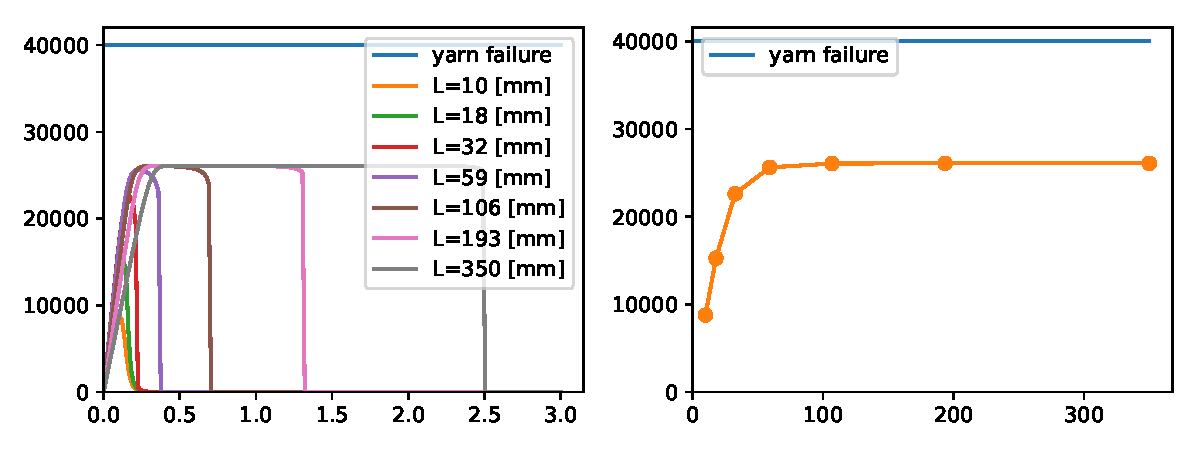
\includegraphics[width=0.95\textwidth]{examples/e51_length_dependence/fig_length_dependence.pdf}\\
    Response for varied fracture energy $G_\mathrm{F} \in [0.01, 0.04, 0.07]$\\
        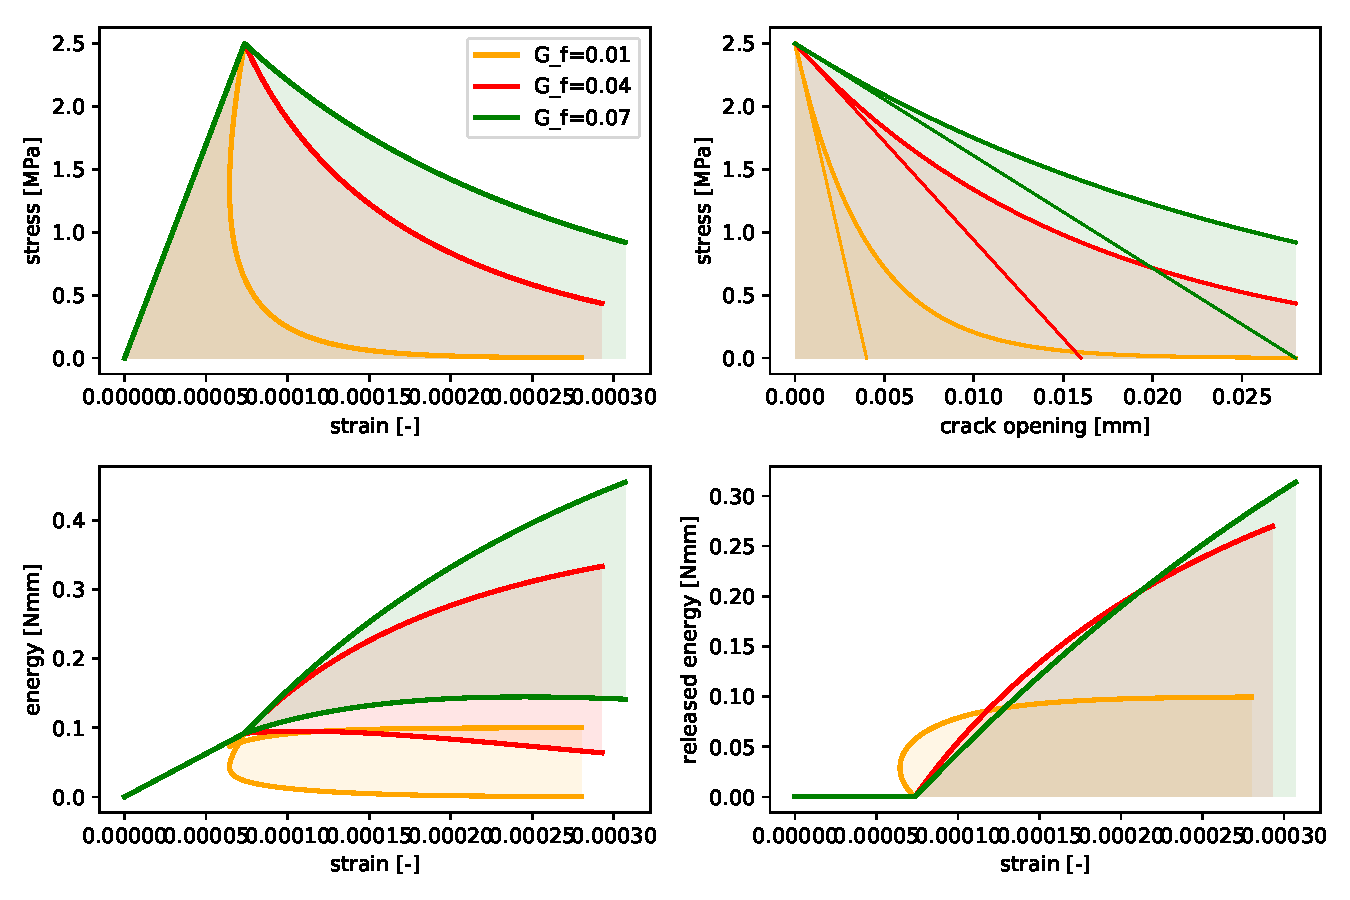
\includegraphics[width=0.95\textwidth]{examples/e51_length_dependence/fig_fracture_energy_dependence.pdf}\\
        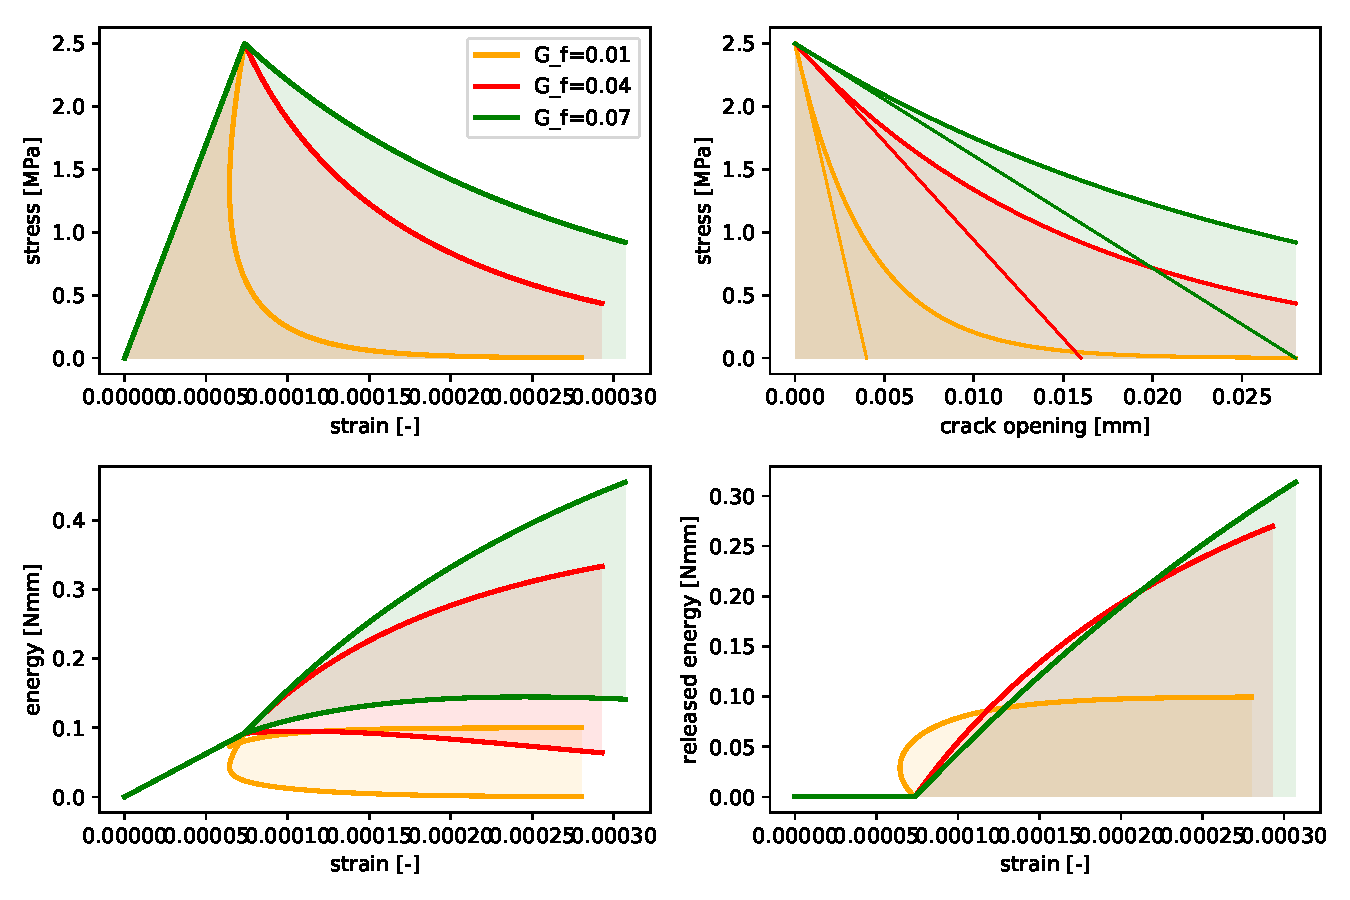
\includegraphics[width=0.95\textwidth]{examples/e51_length_dependence/fig_fracture_energy_dependence.pdf}\\
    \end{center}
\end{center}
            \end{bmcsex}
\end{document}
    